\documentclass[review]{elsarticle}

\usepackage{hyperref}
\usepackage{amsmath}
\usepackage{graphicx}
\usepackage{booktabs}
\usepackage{url}
\usepackage{caption}
\usepackage{siunitx}
\usepackage{geometry}
\usepackage{multirow}
\usepackage{listings}

\journal{Environmental Modelling \& Software}

\begin{document}

\begin{frontmatter}

\title{WS3: An open-source Python framework for integrated simulation and optimization of forest landscape and wood supply systems}

\author[ubc]{Gregory Paradis\corref{cor1}}
\cortext[cor1]{Corresponding author: gregory.paradis@ubc.ca}
\address[ubc]{Faculty of Forestry, University of British Columbia, Canada}

% Highlights (3--5 bullets)
\section*{Highlights}
\begin{itemize}
  \item An open-source Python framework for decision support in forest landscape and wood supply planning.
  \item Modular architecture with solver-backed optimization and hybrid spatial/aspatial workflows.
  \item Interoperable with standard geospatial formats and supports carbon accounting via libcbm.
  \item Reproducible workflows, CI-tested codebase, and PyPI distribution.
  \item Illustrated through reproducible use-case demonstrations with transparent, reusable notebooks and scripts.
\end{itemize}

% Graphical abstract (optional)
\begin{graphicalabstract}
 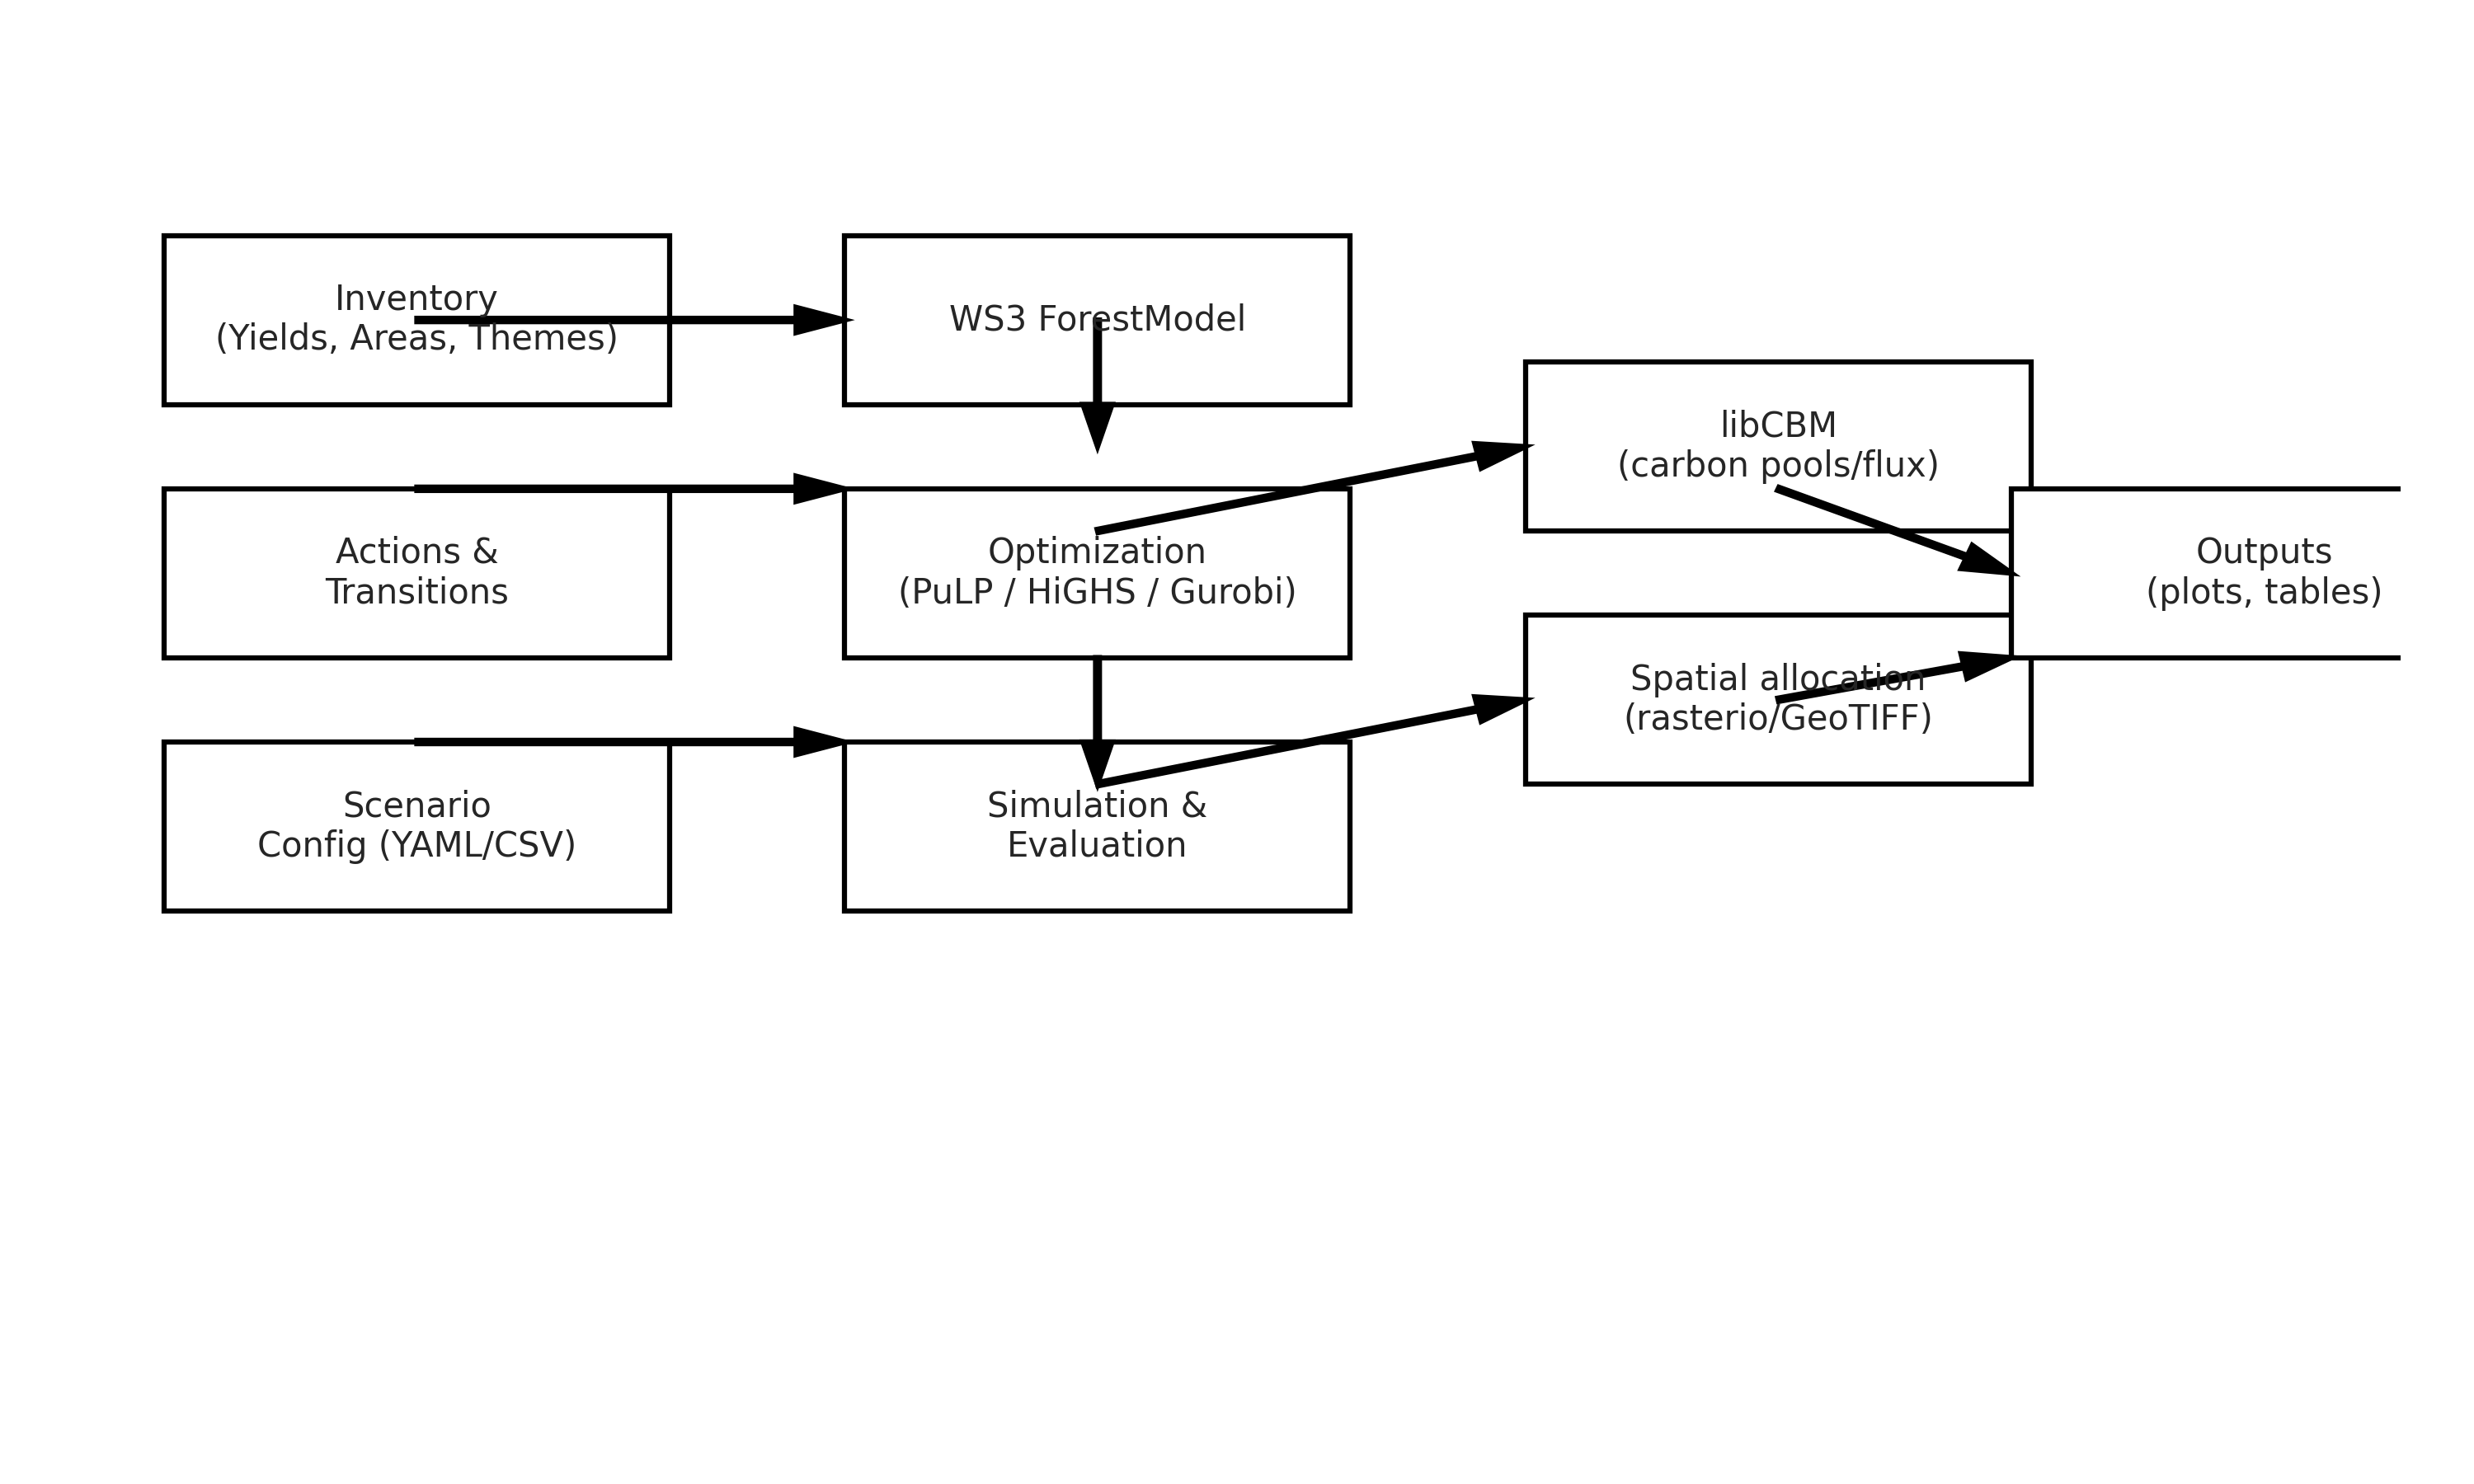
\includegraphics[width=\linewidth]{figs/graphical_abstract.png}
\end{graphicalabstract}

\begin{abstract}
Transparent, reproducible decision support for forest landscape planning increasingly requires integrated treatment of harvest scheduling, spatial allocation, and greenhouse gas (GHG) accounting. We present WS3, an open-source Python framework for long-horizon wood supply modeling that combines modular simulation with solver-backed optimization and hybrid spatial/aspatial workflows. WS3 represents stands, actions, and transitions through a clear data model, supports scenario-based analyses, and interoperates with geospatial rasters for spatial allocation of aspatial schedules. A key contribution is a built-in linkage to the open-source Canadian Forest Service Carbon Budget Model (libCBM), enabling seamless carbon stock and flux estimation alongside traditional harvest and area outcomes. We demonstrate WS3 through reproducible use-case demonstrations that couple optimization-driven harvest scheduling with libCBM carbon accounting and a raster allocation step to visualize spatial implications. These demonstrations highlight how alternative policy constraints influence harvest flows and carbon dynamics, illustrating the framework’s utility for climate change mitigation planning. The full code, documentation, and notebooks are publicly available via GitHub and PyPI, with a versioned archive on Zenodo \citep{ws3_zenodo2025}, and a complete reproduction package accompanying this article. WS3 lowers barriers to rigorous, extensible analysis, supporting researchers and practitioners seeking open, auditable workflows for forest sector planning under evolving climate and policy objectives.
\end{abstract}

\section*{Software availability}
\begin{itemize}
  \item Software name: WS3 (Wood Supply Simulation and Scheduling)
  \item Developers: Gregory Paradis (UBC FRESH) with contributions from the FRESH lab community
  \item First public release: 2015 (v0.1); current version: 1.0.4
  \item Programming language: Python (>=3.9); optional extras: libcbm, PuLP, gurobipy
  \item Source: \url{https://github.com/UBC-FRESH/ws3}; Issue tracker and discussions hosted on GitHub
  \item Distribution: PyPI package \texttt{ws3} (\texttt{pip install ws3} or \texttt{ws3[cbm]}) with wheels for Linux, macOS, Windows
  \item Documentation: \url{https://ws3.readthedocs.io}
  \item Archive: Zenodo release \citep{ws3_zenodo2025} (DOI \href{https://doi.org/10.5281/zenodo.17219651}{10.5281/zenodo.17219651})
  \item License: MIT
\end{itemize}

\begin{keyword}
Environmental modelling \sep Decision support \sep Forest estate \sep Optimization \sep Simulation \sep Spatial modelling \sep Reproducibility \sep Open-source software
\end{keyword}

\end{frontmatter}

\section{Introduction}

Forested landscapes now sit at the centre of intertwined climate mitigation, biodiversity, and bioeconomy mandates, and planners are being asked to reconcile wood supply security with measurable reductions in greenhouse-gas emissions across multi-decadal horizons \citep{canadell2022wgiii, griscom2017natural, fao2020fra}. Meeting these expectations demands decision-support systems that can span harvest scheduling, regeneration and silviculture options, spatial footprint analysis, and explicit carbon accounting, all while remaining transparent enough for regulators, Indigenous governments, and industrial partners to audit \citep{law2018land, smyth2020climate}. The resulting analytical load has outgrown the ad hoc spreadsheets and siloed software stacks still common in practice, underscoring the need for integrated, reproducible modelling platforms that uphold emerging open-science norms such as the PERFICT principles for predictive ecology \citep{hampton2015tao, lowndes2017path, mcintire2022perfict}.

Strategic forest planning has long relied on operations-research formulations such as Model~I path scheduling and its variants, which underpin allowable-cut analyses and forest estate studies worldwide \citep{johnson1977techniques, gunn2007models}. In practice these ideas are delivered through proprietary toolchains---Remsoft Woodstock, Patchworks, FPS-Atlas, JLP (MELA), and Heureka among others---that package data models, solvers, and reporting inside closed desktop environments \citep{remsoft_woodstock, patchworks, fps_atlas, jlp_mela, heureka}. While these systems are mature and widely trusted, their licensing, opaque configuration formats, and limited automation support constrain transparency, collaborative extension, and reproducible research workflows increasingly required by regulators and journals \citep{hampton2015tao}.

In response, an open-source ecosystem has begun to chip away at these constraints. Spatial simulation platforms such as SpaDES and LANDIS-II, scenario-management frameworks like SyncroSim, and integrative planning prototypes such as PRISM demonstrate strong community appetite for modular, shareable tooling \citep{spades, landisii, syncrosim, nguyen2022prism}. SpaDES in particular mirrors WS3's open-science commitments---the core team helped write the PERFICT guidance---yet, by design, it delivers a coordination shell that depends on user-supplied simulation modules for every landscape process. That architecture excels at orchestrating high-fidelity spatial and stochastic dynamics, but the developers themselves acknowledge that harvest modules rarely move beyond stylised heuristics. They have therefore started collaborating with us on a \texttt{spades\_ws3} wrapper so SpaDES users can bring professional-grade wood-supply scheduling into cumulative-effects experiments. LANDIS-II and SELES occupy similar ecological-simulation niches but remain harder to adapt for rigorous forest-estate analysis: LANDIS-II's governance, C\# codebase, and Windows-centric binaries slow outside contributions and impede deployment to linux-based cloud or HPC environments, while SELES is closed-source black-box commercial software whose advanced modules typically require direct support from its original developer. In practice, practitioners must still bolt on their own solver integrations, carbon-accounting pipelines, and spatial reporting to assemble a full decision-support stack \citep{daigneault2022forest, law2018land}. This persistent gap between open landscape-simulation scaffolds and purpose-built forest-estate planning motivates the deterministic, optimization-first framework we introduce with WS3 in the following section.

WS3 fills this methodological gap with a fully open Python framework that preserves the expressive power of legacy Model~I scheduling while embedding reproducibility, automation, and carbon accounting as first-class design goals. It imports Woodstock-format text files to protect historical investments, provides solver-agnostic optimization through PuLP/HiGHS with optional Gurobi, couples natively to the Canadian Forest Service’s libCBM implementation, and exposes hybrid spatial–aspatial workflows compatible with geospatial rasters and SpaDES-based simulations \citep{remsoft_woodstock, pulp, highs, gurobi, kurz2009cbm, libcbm_py, spades}. The codebase embraces open-science practices—version control, packaged releases, and documented reproduction scripts—to support transparent collaboration across institutions \citep{hampton2015tao, lowndes2017path}.

The remainder of this article details the WS3 architecture and data model (Section~2), demonstrates a reproducible use-case workflows linking solver-backed optimal harvest scheduling to libCBM carbon accounting and spatial disturbance allocation for hypothetical linkage to downstream raster-based spatial simulation models (Section~3), discusses impact and reusability (Section~4), compares WS3 with alternative tools (Section~5), and summarises availability, authorship, and future work to facilitate uptake. Together these sections document (i) the design principles and modular implementation of WS3, (ii) an end-to-end workflow that pairs optimization with carbon analysis and spatial outputs, and (iii) comparative evidence and resources that support reuse by researchers and practitioners.

\section{Software description}
\subsection{Architecture}
WS3 implements a modular architecture organized around five roles: (i) core data abstractions; (ii) forest model construction and simulation; (iii) optimization; (iv) spatial allocation; and (v) common utilities. The main modules are:
\begin{itemize}
  \item forest: defines the ForestModel and core abstractions for development types (dtypes), actions, transitions, yields, and scenario compilation. A scenario is specified by a planning horizon, period length, an initial inventory (areas by dtype and age), and transition rules governing state changes under actions and growth.
  \item opt: provides a solver-agnostic interface to formulate linear programming harvest-scheduling problems (objective, variables, constraints) and to solve them using PuLP/HiGHS by default, with optional Gurobi.
  \item spatial: implements utilities to map aspatial schedules to rasters (e.g., GeoTIFF) for visualization and spatial policy evaluation (hybrid spatial/aspatial workflow).
  \item core/common/financial/forest\_helper: shared utilities for interpolation and curves, convenience helpers for examples, and optional financial indicators.
\end{itemize}

\subsubsection{Data model and workflow}
The ForestModel is organized around discrete time (planning periods) and discrete age classes per dtype. Dtypes are keyed by tuples of theme values (e.g., analysis unit, leading species, site class), enabling masks for selective compilation and scheduling. Yields are represented by curves/interpolators, and actions (e.g., harvest, planting, fuel treatment, fire) expose operability and transitions (age reset, dtype change, growth updates). WS3 builds a state-transition tree per dtype across periods. Users can: (i) schedule heuristically using area-control selectors (e.g., Greedy oldest-first), or (ii) schedule optimally via a path-based linear program. Indicators are compiled as:
\begin{itemize}
  \item Action-dependent flows via \texttt{compile\_product(period, expr, acode=...)} (e.g., harvested volume using a utilization-adjusted expression on the total volume yield).
  \item Inventory stocks via \texttt{inventory(period, yname=...)} (e.g., growing stock).
\end{itemize}

\subsubsection{Interoperability}
WS3 can import Woodstock-format text sections (LAN/ARE/YLD/ACT/TRN), enabling reuse of established data pipelines. For carbon, ForestModel exposes \texttt{to\_cbm\_sit} to export Standard Input Table (SIT) configuration/tables consumable by libCBM, with user-provided disturbance-type mappings and per-dtype last-pass-disturbance metadata. Geospatial I/O uses standard formats (shapefile, GeoTIFF). All tabular inputs are plain text (CSV/TSV), and workflows are scripted or notebook-based for reproducibility.

Figure~\ref{fig:architecture} summarizes modules and data flow; Figure~\ref{fig:workflow} outlines the end-to-end case-study workflow used later in the manuscript.

\begin{figure}[h]
  \centering
  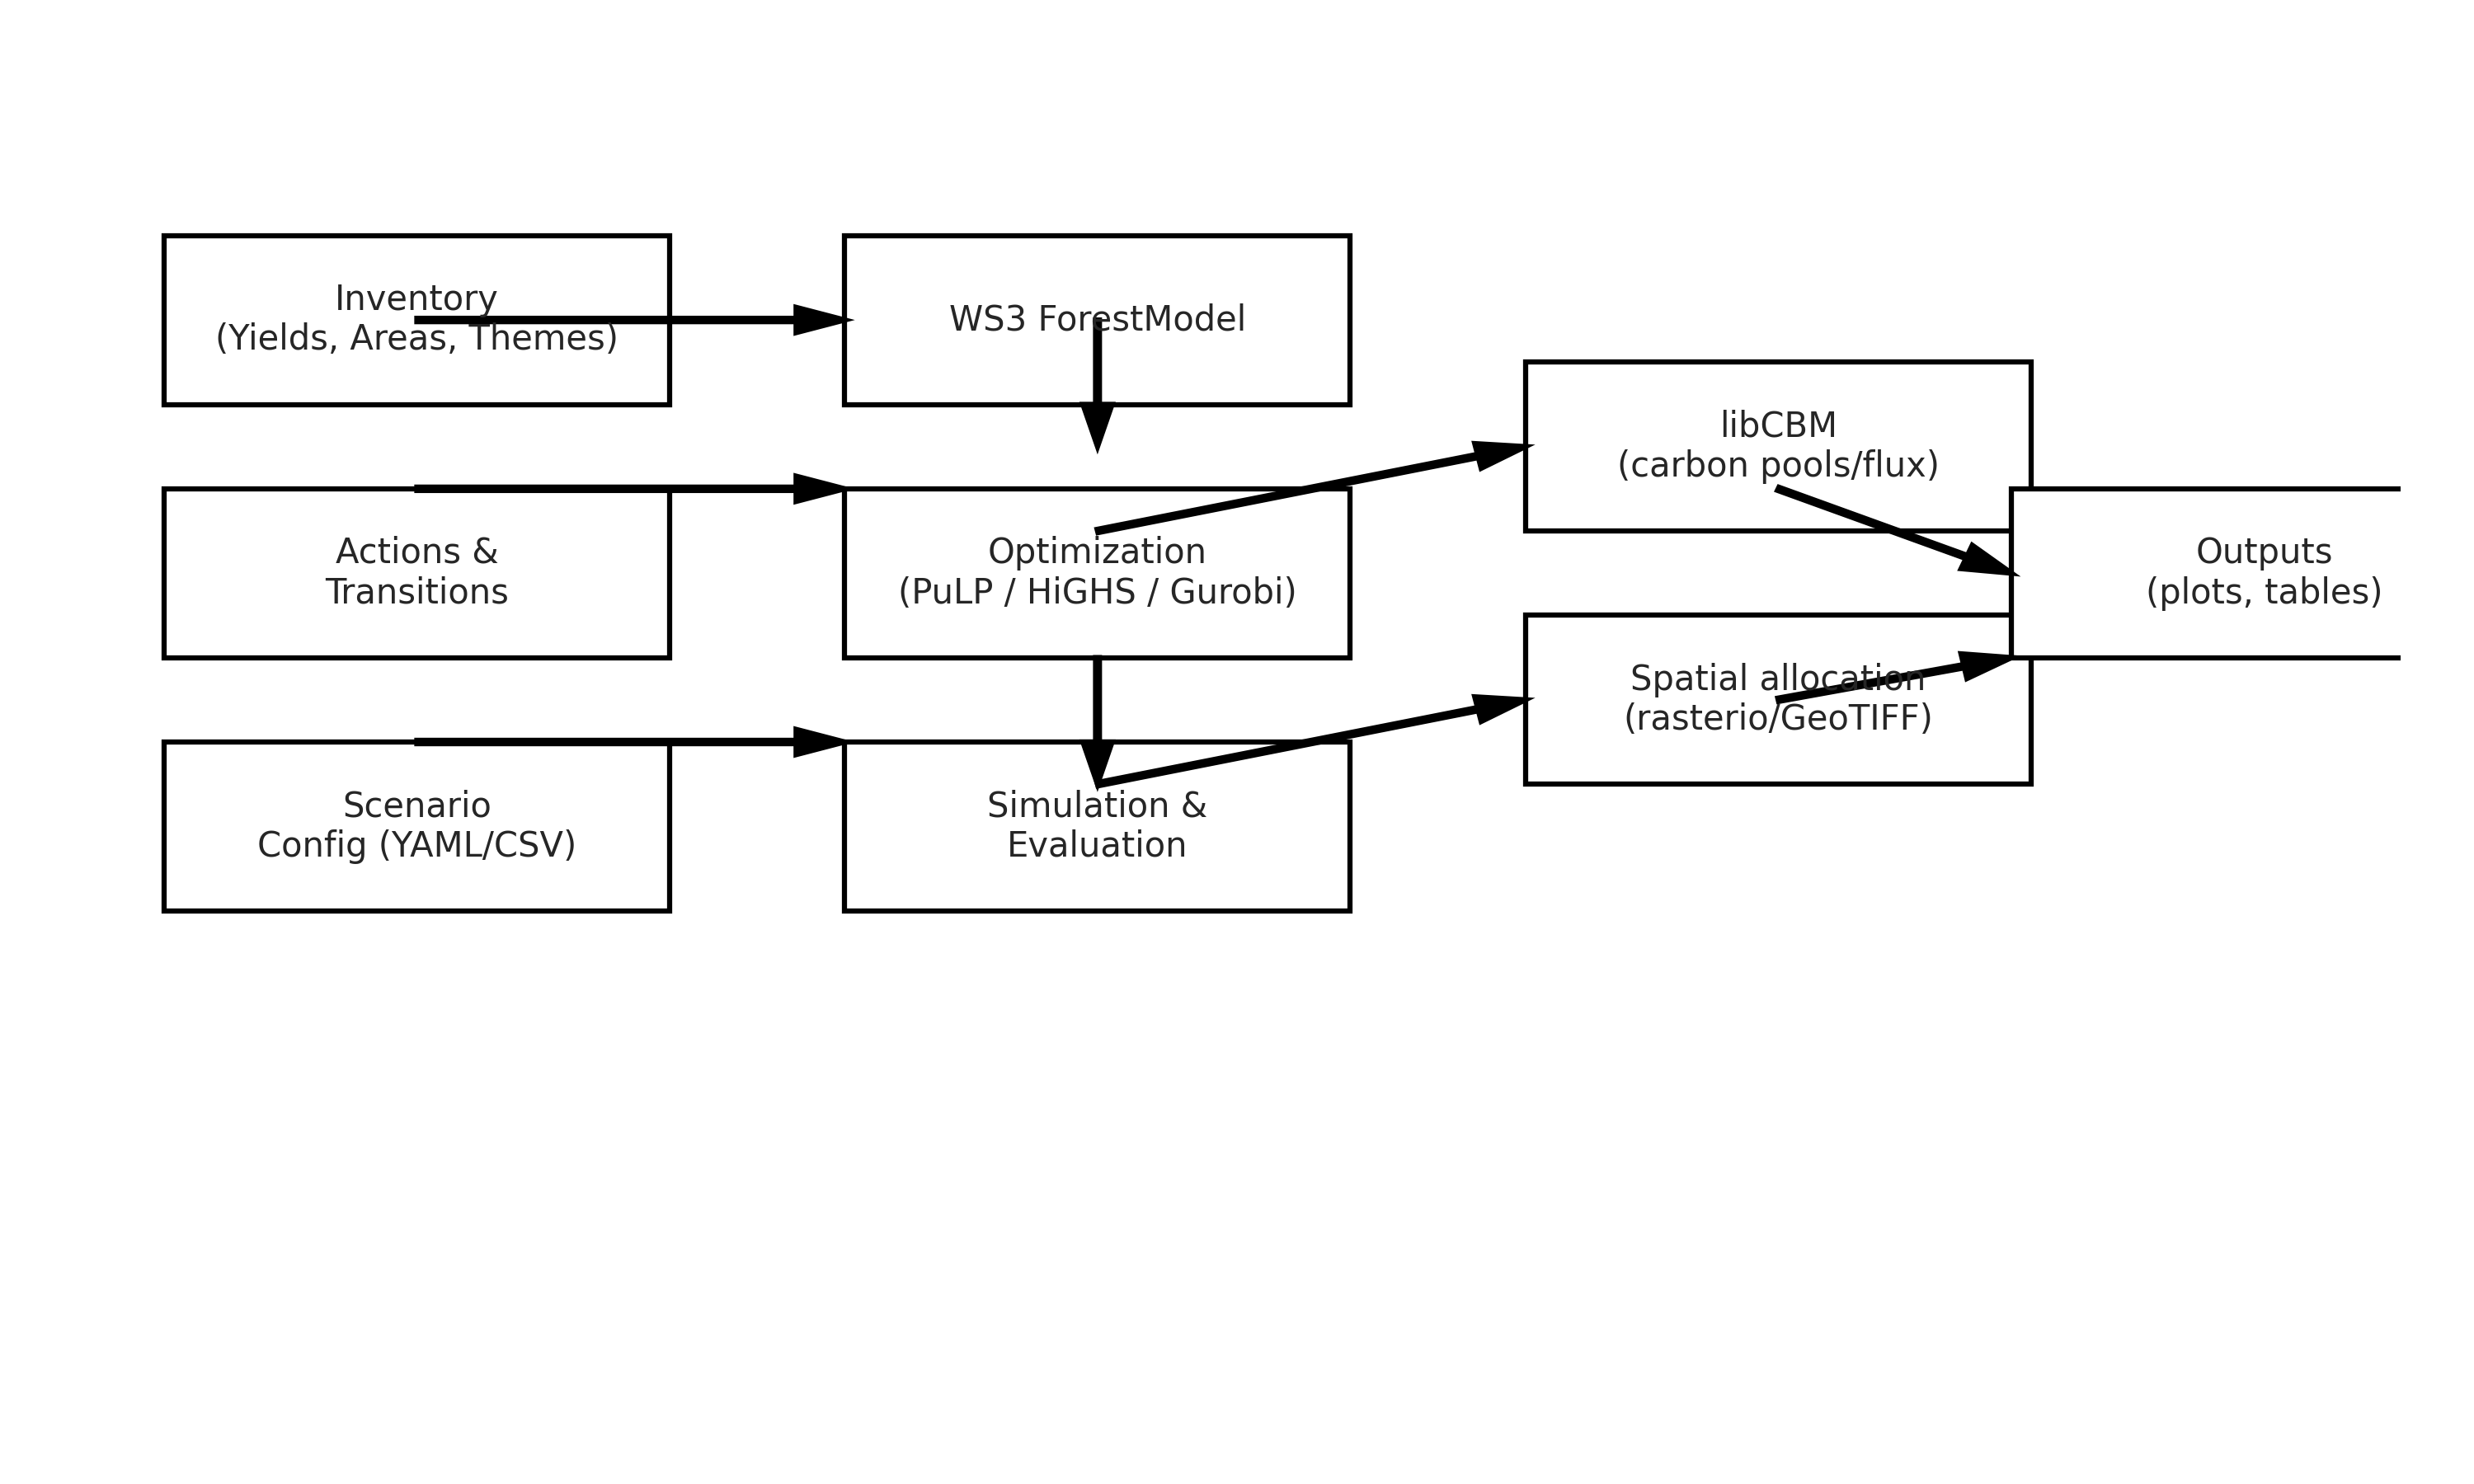
\includegraphics[width=0.95\linewidth]{figs/f1_architecture.png}
  \caption{WS3 architecture: inputs feed a ForestModel; scenarios are scheduled via heuristic or LP; results feed libCBM and optional spatial allocation; plots/tables generated for analysis.}
  \label{fig:architecture}
\end{figure}

\begin{figure}[h]
  \centering
  
\includegraphics[width=0.95\linewidth]{figs/f2_workflow.png}
  \caption{Case study workflow: load inputs, build ForestModel, schedule, export SIT (to\_cbm\_sit), run libCBM, generate plots and tables.}
  \label{fig:workflow}
\end{figure}

\begin{figure}[t]
  \centering
  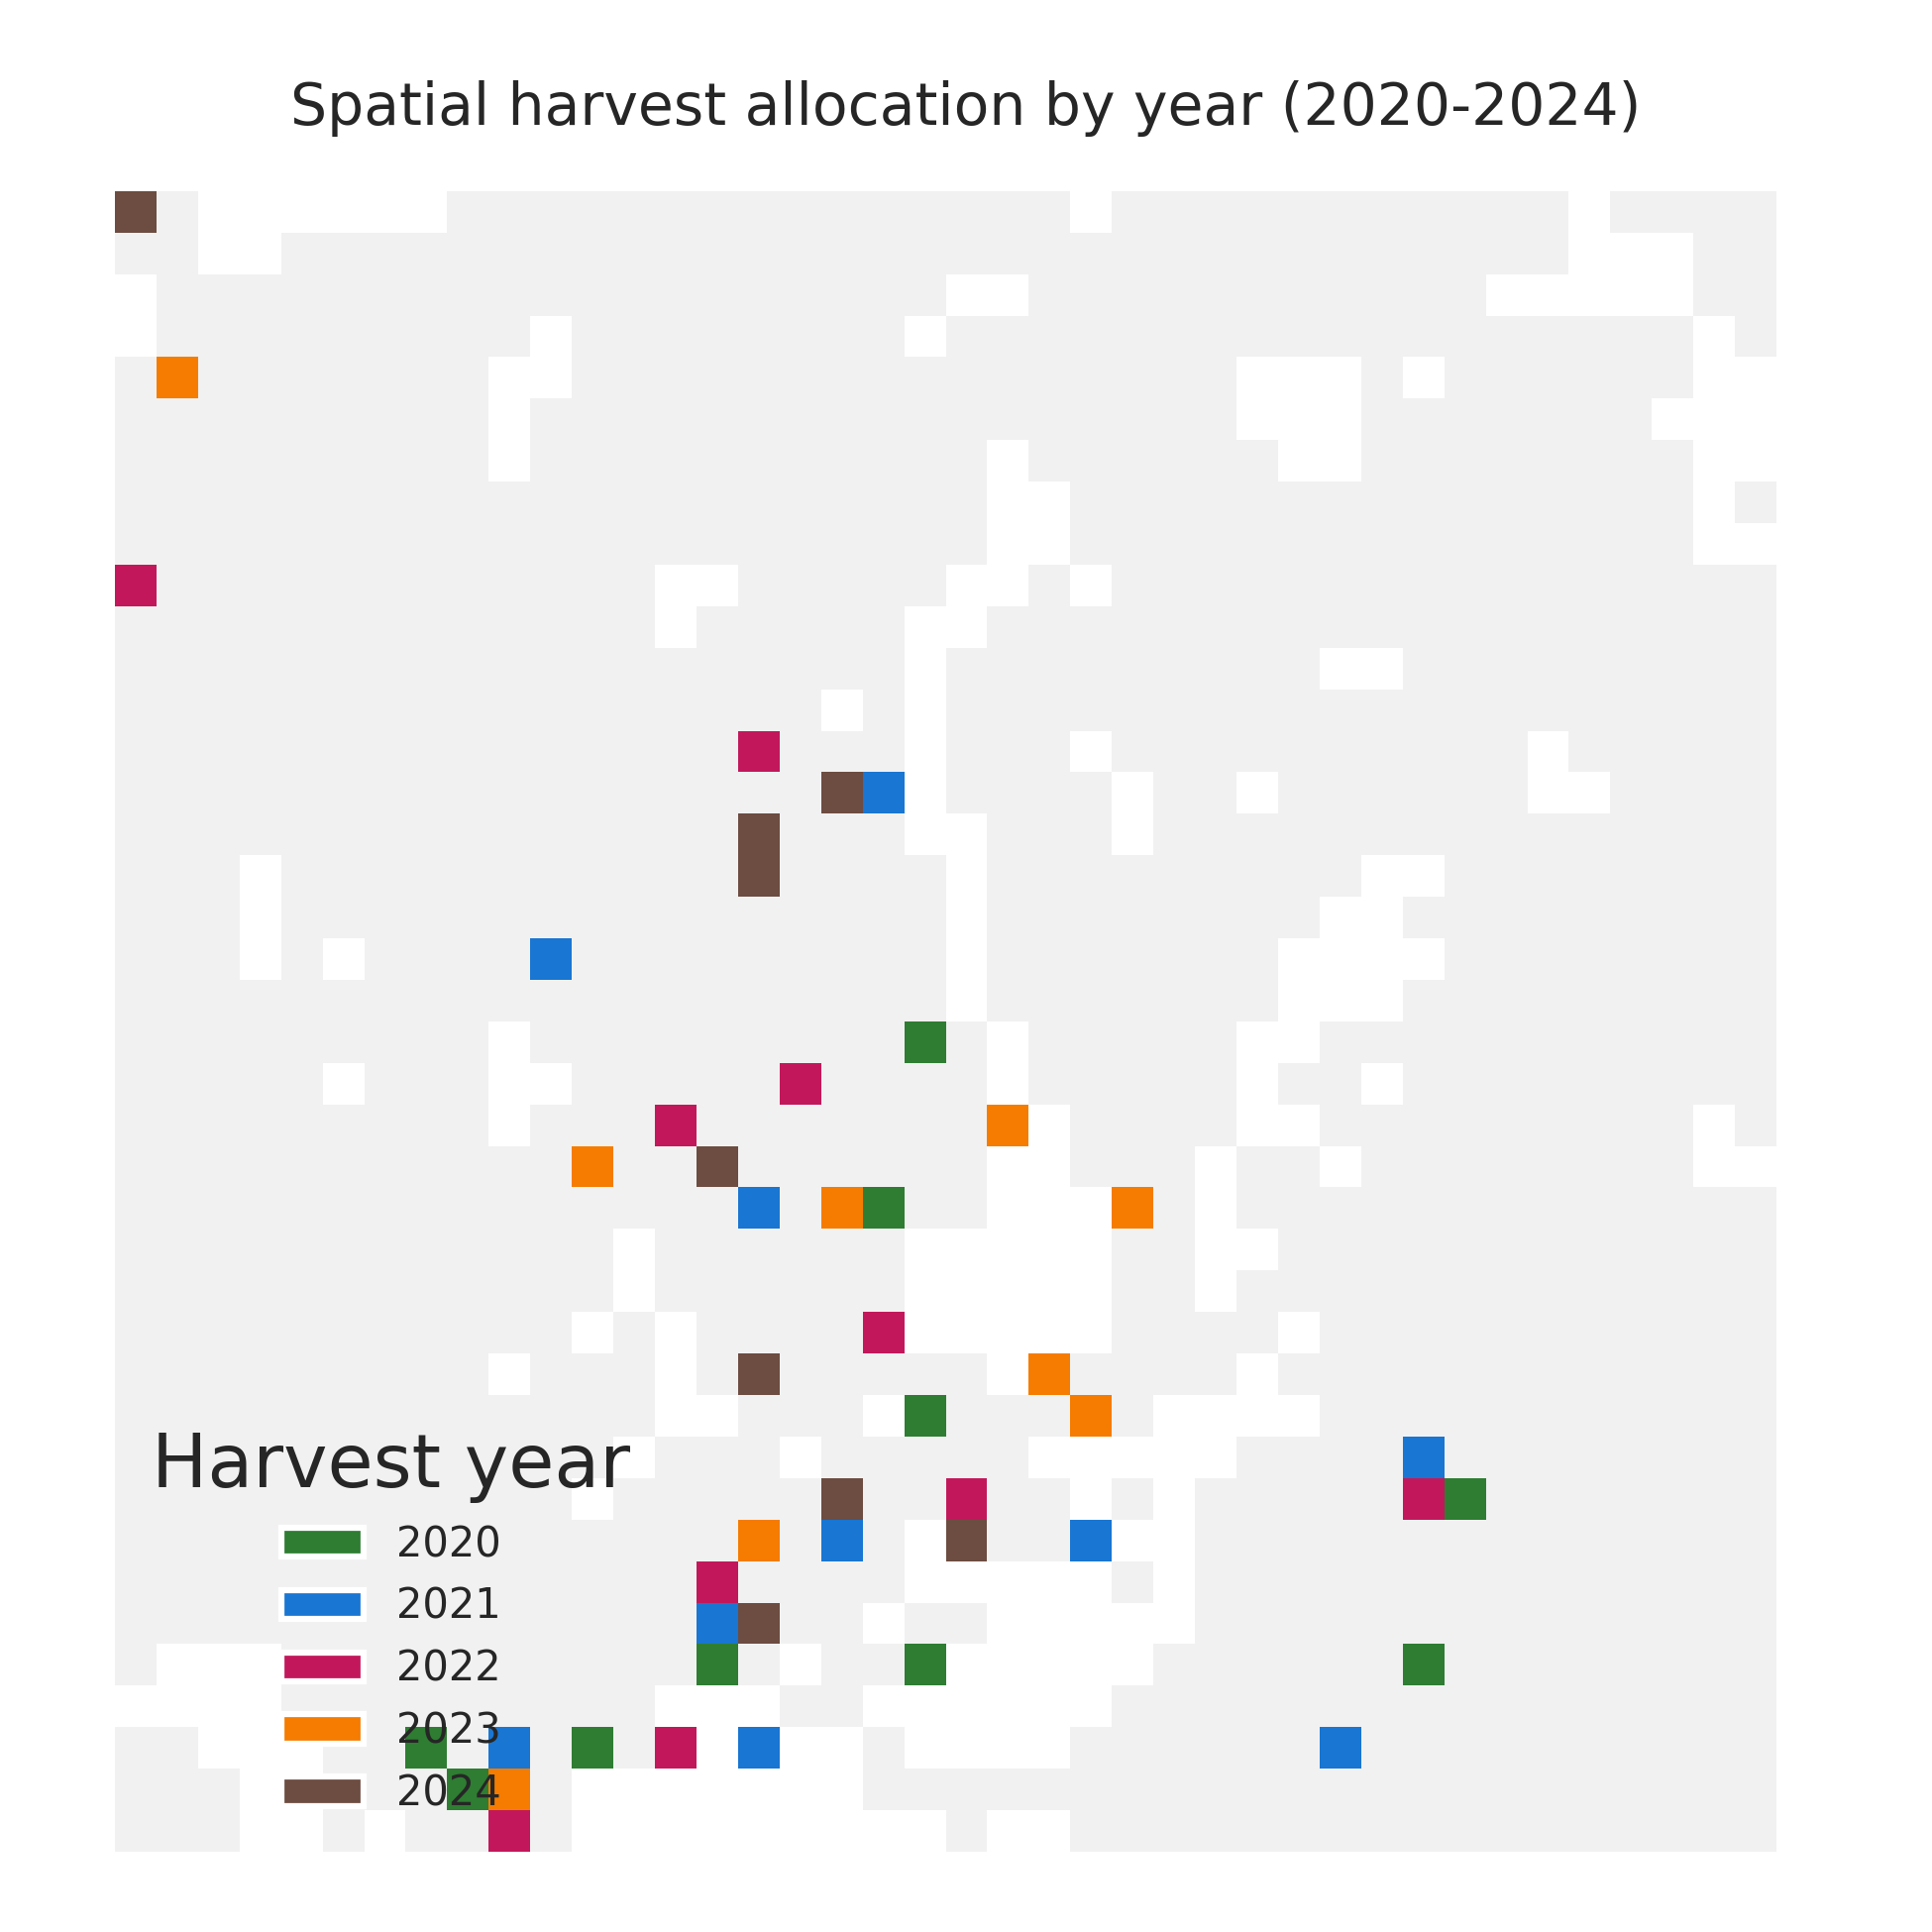
\includegraphics[width=0.7\linewidth]{figs/f3_spatial_allocation.png}
  \caption{Heuristic schedule allocated to space for the 2020--2024 planning window. Colours denote the first year a cell is harvested, overlaid on the full inventory extent (light grey).}
  \label{fig:spatial_allocation}
\end{figure}

\subsection{Optimization formulation (Model I)}
WS3 adopts a path-based Model~I linear program \citep{johnson1977techniques, gunn2007models} in which each decision variable selects the proportion of a spatial zone (dtype) allocated to a feasible root-to-leaf prescription (path) across the planning horizon. Let:
\begin{align*}
  I &: \text{ set of spatial zones (dtypes)} \\
  J_i &: \text{ set of feasible prescriptions (paths) for zone } i\in I \\
  O &: \text{ set of outputs (e.g., harvest area, harvest volume, growing stock, habitat)} \\
  O'&\subseteq O: \text{ targeted outputs subject to even-flow constraints} \\
  T &: \text{ set of planning periods} \\
  T'_p&\subseteq T: \text{ periods on which even-flow for output } p\in O' \text{ is enforced}
\end{align*}
Decision variables are proportions:
\[
x_{ij}\in[0,1] \quad \text{for all } i\in I,\, j\in J_i,
\]
meaning ``the fraction of zone $i$ assigned to prescription $j$''. Let $\mu_{ijot}$ denote the quantity of output $o\in O$ in period $t\in T$ produced by allocating $x_{ij}$ to path $j\in J_i$ for zone $i\in I$. Define a reference-period level $y_p:=\sum_{i\in I}\sum_{j\in J_i}\mu_{ijpt_p^R}x_{ij}$ for each targeted output $p\in O'$ at $t_p^R\in T$, and $\varepsilon_p$ as the allowable even-flow tolerance. With general lower/upper bounds $v^-_{ot},v^+_{ot}$ on outputs, the Model~I LP is:
\begin{align}
\text{maximize}\quad
& \sum_{i\in I}\sum_{j\in J_i} c_{ij}\,x_{ij} \label{eq:ws3_obj}\\
\text{subject to}\quad
& (1-\varepsilon_p)\,y_p \le \sum_{i\in I}\sum_{j\in J_i}\mu_{ijpt}\,x_{ij} \le (1+\varepsilon_p)\,y_p, && \forall p\in O',\, \forall t\in T'_p \label{eq:ws3_evenflow}\\
& v^-_{ot} \le \sum_{i\in I}\sum_{j\in J_i}\mu_{ijot}\,x_{ij} \le v^+_{ot}, && \forall o\in O,\, \forall t\in T \label{eq:ws3_bounds}\\
& \sum_{j\in J_i} x_{ij} = 1, && \forall i\in I \label{eq:ws3_coverage}\\
& 0 \le x_{ij} \le 1, && \forall i\in I,\, \forall j\in J_i. \label{eq:ws3_box}
\end{align}
The objective coefficients $c_{ij}$ encode the user-defined value of a path (e.g., total or discounted volume, revenues, multi-criteria scores). Constraints (\ref{eq:ws3_evenflow}) enforce even-flow on targeted outputs, (\ref{eq:ws3_bounds}) set general lower/upper bounds per period, (\ref{eq:ws3_coverage}) ensures convex mixing of paths to fully cover each zone, and (\ref{eq:ws3_box}) bounds variables as proportions. In WS3, $\mu$-coefficients arise from replaying each path through the simulator, calling \texttt{compile\_product} (for action-dependent outputs like harvest area/volume) or \texttt{inventory} (for stocks like growing stock). The LP matrix is extremely sparse because each path contributes to a limited set of outputs and periods.

Code-to-math mapping. WS3 exposes a coefficient-function pattern that compiles objective and constraint rows from paths. For example, helper functions like \texttt{cmp\_c\_z} (objective), \texttt{cmp\_c\_caa} (action-based flows), and \texttt{cmp\_c\_ci} (inventory-based constraints) traverse path nodes (period, action code, dtype key, age), evaluate the corresponding $\mu$-like contributions via \texttt{compile\_product}/\texttt{inventory}, and assemble the LP using \texttt{fm.add\_problem(...)}. Users select the solver (HiGHS by default; Gurobi optional) and solve via the standard PuLP interface. Upon optimality, WS3 compiles and applies the schedule, then re-simulates to produce indicators for analysis.

Design implications. This path-based Model~I approach embeds intertemporal feasibility in each column, separates simulation from optimization, and enables straightforward addition of new outputs/constraints by supplying new coefficient functions. It also aligns with established forest-planning literature while remaining solver-agnostic and highly sparse for scalability.

\subsection{Implementation}
\emph{Technology stack.} WS3 is implemented in Python and distributed via PyPI. Optimization problems are formulated with PuLP \citep{pulp} and solved with open-source HiGHS \citep{highs} by default, with optional Gurobi \citep{gurobi} for larger instances. Geospatial I/O uses rasterio/fiona/GeoPandas. Documentation (Sphinx) and continuous integration ensure API consistency, example executability, and unit testing.

\emph{libCBM integration.} The ForestModel exposes a to\_cbm\_sit method that compiles a SIT configuration and tables (classifiers, inventory, yields, disturbance events, transitions) consumable by libCBM. Users provide a disturbance type mapping and last-pass disturbance metadata to ensure correct dead organic matter (DOM) spin-up. The sequential demonstration runs libCBM for 200 years using the official Python API and documentation \citep{libcbm_py_docs, libcbm_py_repo}.

\emph{Reproducibility and packaging.} The repository includes examples and a reproduction package (papers/ems/repro) with pinned requirements and scripts to generate all figures and tables. Versioned releases are archived on Zenodo \citep{ws3_zenodo2025}. WS3 supports interactive (Jupyter) and batch (Linux) workflows.

\subsection{Quality assurance and benchmarking}
\emph{Automated testing.} WS3 ships with a pytest suite that exercises the common, core, financial, forest, and optimization modules (29 tests). The suite runs in approximately 4~s on a Linux workstation (Python~3.12) and is executed for every push and pull request via a GitHub Actions workflow (Ubuntu, Python~3.10) that also regenerates a coverage badge \citep{ci_workflow}. Style tooling (black, ruff) is bundled in \texttt{requirements-dev.txt} and wired into the development makefile, ensuring consistent formatting before release.

\emph{Case-study repro checks.} The EMS reproduction package encapsulates the sequential WS3$\to$libCBM pipeline in \texttt{make\_repro.sh}. On the reference workstation (Ubuntu~22.04, 32~GB RAM), the script completes in 6.1~s, re-creating Figures~\ref{fig:flows}--\ref{fig:cbm}, Figure~\ref{fig:spatial_allocation}, and the tables stored in \texttt{papers/ems/tables}. The workflow is deterministic: running \texttt{generate\_case\_study.py} a second time produces byte-identical CSV and PNG assets, providing an integration test for the scheduling, SIT export, and libCBM coupling.

\emph{Performance spot checks.} The heuristic scheduler used in the case study produces a 100-year plan in under a second, and the subsequent 200-year libCBM simulation dominates total runtime (\textasciitilde5~s). Larger linear programs formulated through \texttt{ws3.opt} benefit from HiGHS (default) or optional Gurobi: internal regression notebooks (e.g., Examples~030/040) routinely solve tens-of-thousands-of-stand path-based instances within minutes using HiGHS, while the optional Gurobi backend shortens solve time further via its advanced presolve and feasibility tools. Raster allocations scale linearly with the number of cells processed per period and are trivially parallelisable.

\section{Illustrative use-case demonstrations}
We open with a two-stage sequential pipeline demonstration that first schedules harvest in WS3 and then evaluates carbon dynamics using libCBM. The workflow replicates the existing example 031\_ws3\_libcbm\_sequential-builtin.ipynb to ensure full reproducibility.

\emph{Study design.} We use the public example dataset \texttt{tsa24\_clipped} provided with WS3. The inputs are stored as Woodstock-format text files (landscape, areas, yields, actions, transitions) under \texttt{examples/data/woodstock\_model\_files} and imported into a \texttt{ForestModel}. We then schedule harvest using a self-parameterizing area-control heuristic to produce an aspatial action schedule over a 100-year horizon (10 periods of 10 years), and finally export a libCBM Standard Input Table (SIT) to simulate annual carbon stocks and fluxes.

\emph{Data and study area.} The \texttt{tsa24\_clipped} dataset is a clipped subset of a Timber Supply Area inventory used for demonstration. The initial inventory enumerates development types (dtypes) by theme tuples (e.g., analysis unit, species, site), with associated yield curves for total volume (\texttt{totvol}) and species-volume splits (\texttt{swdvol}, \texttt{hwdvol}). Actions and transitions define operability and state changes (e.g., harvest resets age).

\emph{Model setup and scheduling.} We initialize the model with \texttt{base\_year}=2020, \texttt{horizon}=10, \texttt{period\_length}=10\,y, and \texttt{max\_age}=1000. After importing sections and initializing areas, we add a null action and reset actions. The area-control scheduler selects target areas by mask (default: AU-wise THLB) and applies actions using a priority-queue selector (oldest-first). Target areas are computed from area-weighted mean CMAI ages; utilization is set to 0.85 in the volume expression used for compiled flows. The resulting schedule is compiled and applied to produce period-by-period flows and stocks.

\emph{libCBM coupling and metrics.} We define a disturbance-type mapping for actions (harvest$\to$Clearcut harvesting without salvage; fire$\to$Wildfire) and assign \texttt{last\_pass\_disturbance} per dtype to ensure consistent DOM spin-up. Using \texttt{ForestModel.to\_cbm\_sit} with softwood and hardwood volume names (\texttt{swdvol}, \texttt{hwdvol}), \texttt{admin\_boundary} = \texttt{"British Columbia"}, and \texttt{eco\_boundary} = \texttt{"Montane Cordillera"}, we export SIT config and tables. We then run libCBM for \texttt{n\_steps}=200 years, aggregating annual carbon stocks (biomass, DOM, total ecosystem).

\emph{Outputs.} We report time-series of harvested area/volume and growing stock from WS3, and annual carbon stocks from libCBM. The reproduction package generates the figures and tables used below.

The full, deterministic workflow is scripted in \texttt{papers/ems/repro/generate\_case\_study.py}, which produces the flows table and carbon stocks table:
\begin{itemize}
  \item \texttt{papers/ems/tables/scenario\_flows.csv}: harvest area, harvest volume, and growing stock by period.
  \item \texttt{papers/ems/tables/annual\_carbon\_stocks.csv}: annual biomass, DOM, and total ecosystem carbon.
\end{itemize}
\begin{table}[h]
\centering
\caption{Sequential demonstration parameters and configuration (WS3 $\to$ libCBM pipeline).}
\begin{tabular}{p{4.2cm}p{9.5cm}}
\toprule
Setting & Value \\
\midrule
Dataset & \texttt{tsa24\_clipped} (Woodstock-format inputs; \texttt{examples/data/woodstock\_model\_files}) \\
Base year & 2020 \\
Planning horizon & 10 periods (100 years) \\
Period length & 10 years \\
Max age class & 1000 years \\
Yield names & \texttt{totvol} (total volume), \texttt{swdvol} (softwood), \texttt{hwdvol} (hardwood) \\
Scheduling method & Area-control heuristic (priority-queue, oldest-first); utilization 0.85 \\
Disturbance mapping (CBM) & harvest$\to$Clearcut harvesting without salvage; fire$\to$Wildfire \\
CBM export & \texttt{ForestModel.to\_cbm\_sit} (admin: British Columbia; eco: Montane Cordillera) \\
CBM run length & 200 annual steps \\
Outputs & \texttt{scenario\_flows.csv} (periodic flows/stocks); \texttt{annual\_carbon\_stocks.csv} (annual pools) \\
\bottomrule
\end{tabular}
\label{tab:case_params}
\end{table}

Figures~\ref{fig:flows} and \ref{fig:cbm} visualize the resulting flows and carbon stocks. The entire pipeline, including architecture and workflow diagrams (Figures~\ref{fig:architecture}–\ref{fig:workflow}) and the spatial allocation example (Figure~\ref{fig:spatial_allocation}), is reproducible via \texttt{papers/ems/repro/make\_repro.sh}. The libCBM run length (200 years) matches the example and can be adjusted.

\begin{figure}[h]
  \centering
  
\includegraphics[width=0.95\linewidth]{figs/f4a_harvest_and_stock.png}
  \caption{WS3 results: harvested area, harvested volume (utilization-adjusted), and growing stock over planning periods.}
  \label{fig:flows}
\end{figure}

\begin{figure}[h]
  \centering
  
\includegraphics[width=0.95\linewidth]{figs/f4b_carbon_stocks.png}
  \caption{libCBM results: annual carbon stocks (biomass, dead organic matter, total ecosystem) over 200 years.}
  \label{fig:cbm}
\end{figure} 

\emph{Results.} The heuristic scheduler delivers a 10-period harvest plan whose flows stay within \textasciitilde10\% of their period means without any explicit even-flow constraint: harvest area averages 106.8~kha (dataset convention) with a coefficient of variation of 0.047, and harvest volume averages 15.3~Mm$^3$ with a coefficient of variation of 0.106 (Table~\ref{tab:case_params}; Figure~\ref{fig:flows}). Growing stock declines smoothly from 135 to 82 in the same area-equivalent units (consistent with the 0.85 utilization factor), documenting the state trajectory exported to libCBM. In the carbon stage, libCBM aggregates show biomass pools increasing from $2.7\times10^5$~tC to $3.1\times10^5$~tC over 200 years, while DOM remains within $1.7$--$1.9\times10^5$~tC, yielding a total ecosystem carbon gain of 42~ktC (Figure~\ref{fig:cbm}). The summary tables \texttt{scenario\_flows.csv} and \texttt{annual\_carbon\_stocks.csv} (\texttt{papers/ems/tables}) retain the raw outputs for external verification.

\emph{Reproducibility.} This demonstration is intended to be transparent and portable; all input data reside in \texttt{examples/data/woodstock\_model\_files}. The spatial allocation step renders the raster-based harvest allocation shown in Figure~\ref{fig:spatial_allocation}, derived directly from the aspatial schedule via the ForestRaster utility. The folder papers/ems/repro contains \texttt{make\_repro.sh}, which provisions a clean virtual environment, installs pinned dependencies, and runs deterministic scripts that regenerate Figures~\ref{fig:architecture}--\ref{fig:cbm} and the accompanying CSV tables. Outputs are checksum-stable across repeated runs, providing an audit trail for review and reuse.

\subsection*{Broader example library and carbon-aware optimization}
Beyond the sequential carbon-accounting demonstration, WS3 includes a curated set of executable notebooks designed as progressive tutorials, from synthetic examples to realistic policy-oriented analyses. Example 040 showcases carbon-aware optimization by embedding carbon prices and/or constraints directly in the harvest scheduling LP and computing carbon stocks and fluxes with \texttt{libcbm\_py}. A public, end-to-end use-case demonstration exploring carbon-aware scheduling in a stylized British Columbia landscape is available in the repository by Yan (MSc), including scenario automation, sensitivity analysis, and reproducible outputs \citep{yan2025mathematical, yan_repo}.

\begin{figure}[h]
  \centering
  
\includegraphics[width=0.95\linewidth]{figs/f5_neilsonhack_compare.png}
  \caption{Neilson-hack demonstration (Example~040): comparison of libCBM (solid) and WS3-embedded (dashed) carbon indicators after bootstrapping pools/fluxes into WS3 as yield curves. Top: ecosystem carbon pools; Bottom: aggregate decay emissions flux.}
  \label{fig:neilsonhack}
\end{figure}

\section{Impact and reusability}

WS3 enables transparent, auditable analysis for forest landscape planning and climate mitigation, responding to calls for credible natural climate solutions and land-sector mitigation accounting \citep{griscom2017natural, grassi2022historical}. It has supported research on bioenergy \citep{cantegril2019bioenergy}, value-creation potential and supply modelling \citep{paradis2018retro, paradis2018estimating}, and climate impact assessment \citep{smyth2020climate, ke2024climate, yan2025mathematical}. WS3 integrates with the SpaDES ecosystem for spatial simulation \citep{spades} and has been deployed as a backend in decision-support applications. The open MIT license, modular API, and PyPI distribution lower barriers to community contributions and reuse across jurisdictions.

\paragraph{Major use-cases (2015--2025)}
\begin{itemize}
  \item Strategic wood supply and bioenergy planning in mixed-wood forests: optimization and scenario analysis of value-creation options \citep{cantegril2019bioenergy}.
  \item Hybrid simulation--optimization for value indicators and model retrofitting: methods and transfer to production-style analyses \citep{paradis2018retro, paradis2018estimating}.
  \item Climate mitigation and carbon-aware planning in British Columbia: sequential WS3$\to$libCBM pipelines and optimization under policy constraints; graduate theses and applied demonstrations \citep{ke2024climate, yan2025mathematical, yan_repo}.
  \item Decision-support prototypes for nature-based solutions: avoided fire and avoided harvest workflows (Examples 050/060) with net-emission indicators derived from libCBM.
  \item Integration with spatial simulation: \texttt{spades\_ws3} module bridging WS3 with SpaDES for disturbance and landscape dynamics studies \citep{spades, spades_ws3}.
  \item Application backends: WS3 used in web-based decision-support systems (e.g., \texttt{ecotrust\_dss}) for scenario configuration and reporting \citep{ecotrust_dss}.
  \item Ongoing initiatives: CCCANDiES (integrated carbon and ecosystem services; in progress) and mining-sector nature-based solutions (separate paper under review, Journal of Cleaner Production).
\end{itemize}

Interoperability fosters reusability: tabular/text inputs, raster outputs, and the libCBM linkage allow WS3 to slot into existing analytical pipelines. The reproduction package, unit tests, and CI enhance trust and facilitate method transfer, aligned with community guidance on open and efficient scientific practice \citep{hampton2015tao, lowndes2017path}. The architecture is intentionally general, making it applicable to studies of sustainable yield, carbon accounting, biodiversity, and policy trade-offs \citep{boisvenue2022managing}.

\paragraph{Practical impact and reusability highlights}
\begin{itemize}
  \item Openness and packaging: MIT license, PyPI distribution, versioned releases archived on Zenodo \citep{ws3_zenodo2025}; complete examples and tutorials.
  \item Interoperability: Woodstock-format import for legacy/industry pipelines; libCBM SIT export for carbon; standard geospatial formats (GeoTIFF, shapefile).
  \item Reproducibility: deterministic reproduction package (\texttt{papers/ems/repro}) that regenerates all figures/tables; CI runs tests and validates examples.
  \item Extensibility: modular API for adding outputs/constraints and new scheduling logic (heuristic or LP-based); solver-agnostic (HiGHS by default; Gurobi optional).
  \item Integration pathways: SpaDES ecosystem via \texttt{spades\_ws3}; backend for decision-support applications and web services.
  \item Education and onboarding: progressive example notebooks (from \texttt{010} to \texttt{060}) facilitate training and method transfer.
\end{itemize}

An advanced example notebook demonstrates how WS3 can be used to construct a stand-level optimization problem with explicit integration of carbon dynamics using \texttt{libcbm\_py}. This example solves a linear program that balances timber harvest revenues with carbon sequestration benefits under different carbon pricing assumptions (see Example 040). The workflow illustrates how WS3’s optimization layer and libCBM coupling enable carbon-aware planning experiments without bespoke glue code, supporting emerging policy analyses in nature-based climate solutions.

\section{Comparison to alternatives}

\begin{table}[h]
\centering
\caption{Comparison of WS3 with selected tools.}
\begin{tabular}{p{2.5cm}p{2.2cm}p{1.6cm}p{2.3cm}p{2.3cm}p{2.3cm}p{2.2cm}}
\toprule
Tool & Scope & License & Optimization integration & Spatial workflow & Carbon integration & Geography focus \\
\midrule
WS3 & Landscape & Open (MIT) & Built-in (PuLP; optional Gurobi) & Hybrid aspatial-to-raster & Built-in libCBM linkage & General \\
Remsoft Woodstock & Landscape & Proprietary & Built-in & Extensions; connectors & External integrations & General \\
Patchworks & Landscape & Proprietary & Built-in & Spatial planning emphasis & External integrations & General \\
SpaDES & Simulation framework & Open & External packages & Fully spatial (agent-based, raster) & Via modules & General \\
SIMFOR & Stand-level & Open & Limited/none & N/A & Limited/none & General \\
Heureka & Landscape & Mixed/Restricted & Built-in & Spatial capabilities & External integrations & EU-focused \\
JLP (MELA) & Landscape & Restricted/Legacy & Built-in & Spatial extensions & External integrations & Finland-focused \\
\bottomrule
\end{tabular}
\end{table}

\noindent
WS3 differs primarily in its open Python API, explicit libCBM integration, and hybrid spatial/aspatial workflow designed for reproducible research and policy analysis. We emphasize that SIMFOR operates at stand level, while WS3, Woodstock, Patchworks, Heureka, and JLP target landscape-scale planning with varying degrees of spatial explicitness and availability \citep{remsoft_woodstock, patchworks, spades, heureka, jlp_mela, simfor}.

\paragraph{Comparison narrative}
Proprietary landscape systems such as Woodstock and Patchworks provide mature optimization and spatial planning capabilities, but their licensing and closed codebases limit transparent methods development, automated testing, and reproducibility at scale. SpaDES, by contrast, is an open simulation framework oriented to spatial processes and agent-based dynamics; it does not natively provide a solver-backed harvest scheduling layer but interoperates with WS3 via \texttt{spades\_ws3} for hybrid workflows. Heureka and JLP are landscape-oriented and include optimization, yet are region-specific or legacy-maintained, which constrains adoption beyond their primary jurisdictions.

WS3’s distinctive contribution is to combine: (i) a solver-agnostic, path-based Model~I LP generator embedded directly in an open forest estate API; (ii) a documented, first-class linkage to libCBM for carbon stocks and fluxes; and (iii) a hybrid spatial/aspatial pipeline with standard geospatial I/O. These design choices enable reproducible, auditable workflows in notebooks and scripts, fast iteration on objectives/constraints, and easy integration into larger research and decision-support ecosystems. For many research and policy analyses, this balance of openness, extensibility, and end-to-end reproducibility is decisive—even when spatial planning itself is conducted in a specialized tool, WS3 can serve as the transparent scheduling and carbon accounting engine feeding it.

\section{Conclusions and future work}
WS3 provides an open, extensible framework for integrating harvest scheduling, simulation, and carbon accounting. By coupling solver-backed scheduling with libCBM via a documented interface, WS3 supports policy-relevant analyses with transparent, reproducible workflows.

Future work will expand uncertainty handling (stochastic scheduling, sensitivity analysis), add cloud/HPC deployment patterns, and strengthen spatial allocation and visualization. We also plan to enhance carbon–economics linkages and support machine learning surrogates for speedups in large scenario ensembles. The open design invites community extensions and cross-ecosystem applications.

\section*{Code and data availability}
WS3 source code is publicly available at \url{https://github.com/UBC-FRESH/ws3} and distributed via PyPI (\texttt{pip install ws3}). Versioned releases are archived on Zenodo (DOI \href{https://doi.org/10.5281/zenodo.17219651}{10.5281/zenodo.17219651}) \citep{ws3_zenodo2025}. Documentation and tutorials are available at \url{https://ws3.readthedocs.io}. A complete reproduction package for the sequential demonstration, including environment files, scripts, and figure-generation notebooks, is provided as supplementary material and in the release archive.

\paragraph{Reproducibility}
All figures and tables are generated by scripts in \texttt{papers/ems/repro}. The \texttt{make\_repro.sh} script creates an isolated environment, installs pinned dependencies (\texttt{requirements.txt}), and runs \texttt{generate\_diagrams.py}, a spatial schematic stub generator (\texttt{generate\_spatial\_stub.py}), and the sequential demonstration script (\texttt{generate\_case\_study.py}). Outputs are written to \texttt{papers/ems/figs} and \texttt{papers/ems/tables}. The exact versions are preserved via the Zenodo-archived release.

\paragraph{FAIR compliance}
Findable: versioned releases archived with DOI on Zenodo \citep{ws3_zenodo2025} and indexed on GitHub/PyPI. Accessible: open-source license (MIT) and public repository without authentication. Interoperable: open formats for tabular and raster data (CSV, GeoTIFF) and a documented API linking to libCBM. Reusable: pinned environments, CI-tested examples, detailed documentation, and a complete reproduction package accompanying this article.

\section*{CRediT authorship contribution statement}
Gregory Paradis: Conceptualization, Methodology, Software, Validation, Formal analysis, Investigation, Data curation, Writing—original draft, Writing—review \& editing, Visualization, Supervision, Project administration, Funding acquisition.

\section*{Acknowledgements}
Development of WS3 was supported by the Forest Resources Environmental Services Hub (FRESH) at the University of British Columbia. Funding was provided by the Canada Foundation for Innovation (CFI JELF), the British Columbia Knowledge Development Fund (BCKDF), Mitacs, Environment and Climate Change Canada (ECCC), the Natural Sciences and Engineering Research Council of Canada (NSERC), Natural Resources Canada (NRCan), and the Government of British Columbia. The author thanks Elaheh Ghasemi, Salar Ghotb, and Kathleen Coupland for their contributions to documentation, testing, and code quality improvements leading up to this release.

\section*{Declaration of competing interest}
The authors declare no competing interests.

\bibliographystyle{elsarticle-harv}
\bibliography{paper}

\end{document}
